\documentclass[handout,nooutcomes]{ximera}
%\usepackage{wasysym}
\title{Math 160 Lab 1}
\author{Mary E. Pilgrim}

\begin{document}

\section{Math 160 Lab 1 \\ Tolerance}

\begin{abstract}
This is Lab 1 for Math 160 - Due Friday, 27 January, 2017. This lab will cover tolerance and provide an introduction to the idea of limits.

Unless specified otherwise, round decimals to 6 places.
\end{abstract}

\maketitle

%%BALL BEARINGS PROBLEM%%
\begin{problem}{\textbf{\textit{Ball Bearings}}}

You work for a company that manufactures ball bearings. Currently you are working on quality control for ball bearings with ball diameter measuring $10mm$. Now, in the real world, measurements are not perfect...
    %%Part 1a
    \begin{problem}{\textbf{\#1a:}}
    Calculate the ``perfect'' volume of one of these balls.
    $\answer[tolerance=0.000001]{4/3 \pi 5^3}$
    
    What are the units for the ``perfect'' volume?
    \begin{multipleChoice}
    \choice{$mm$}
    \choice{$mm^2$}
    \choice[correct]{$mm^3$}
    \end{multipleChoice}
  
    \end{problem}
    %%Part 1b
    \begin{problem}{\textbf{\#1b:}}
    An order has been placed by a skateboard company. They need ball bearings for some of the wheels they are manufacturing. For wheel assembly, the volume of each ball must be within $1.57mm^3$ of the perfect volume. With this tolerance in mind, what is the largest amount that the radius of each ball can vary from the perfect radius? (a percent SHOULD NOT be given here)
    $\answer[tolerance=0.000001]{(3/4((4/3 \pi 5^3)+1.57)/\pi)^(1/3)-5}$
    \end{problem}
    %%Part 1c
    \begin{problem}{\textbf{\#1c:}}
    You need to put together an order for an aerospace company. For this order there must be less variation in the volume. A variation of $\pm0.03mm^3$ will be tolerated in the volume. Based on this, what is the largest amount of error that the radius of a given ball can have? (a percent SHOULD NOT be given here)
    $\answer[tolerance=0.000001]{(3/4((4/3 \pi 5^3)+0.03)/\pi)^(1/3)-5}$    
    \end{problem}
    
    
    %%Part 1d
    \begin{problem}{\textbf{\#1d:}}
    \textbf{Your answer to this question should be typed or written in a separate document and labeled as Problem 1d.}
    The aerospace company realizes that they can tolerate even less error in the volume of the ball bearings than $\pm 0.03 mm^3$.  Can we repeat the process in \#1c for any arbitrarily small tolerance for error in the volume?  Explain why or why not by referencing the process you carried out in \#1c.
    \end{problem}
\end{problem}

%%CRYSTAL GROWTH PROBLEM%%
\begin{problem}{\textbf{\textit{Crystal Growth}}}

A crystal growth furnace is used in research to determine how best to manufacture crystals used in electronic components for the space shuttle.  For proper growth of the crystal, the temperature must be controlled accurately by adjusting the input power.  Suppose the relationship is given by

\[T(w)= 0.1 w^2 +2.155 w +19.985
\]

where $T$ is the temperature in degrees Celsius and $w$ is the power input in watts.
    %%Part 2a
   \begin{problem}{\textbf{\#2a:}}
   How many watts of power are needed to maintain the temperature at exactly 200$^\circ$ C?
   $\answer[tolerance=0]{33}$
   
   What are the units for the ``perfect'' power needed to maintain the temperature at exactly 200$^\circ$?
    \begin{multipleChoice}
    \choice{degrees Celsius}
    \choice[correct]{watts}
    \choice{$mm^3$}
    \end{multipleChoice}
   \end{problem}
   
   %%Part 2b
   \begin{problem}{\textbf{\#2b:}}
   What interval around the ideal power found in (a) must the power be to keep the temperature within $\pm 1^\circ$C  of the 200$^\circ$C required for proper crystal growth? Be sure to use algebra to show that if the power is kept in this range, the temperature will, indeed, be within $\pm 1^\circ$C  of 200$^\circ$C.
   
   $\answer[tolerance=0.00001]{\sqrt{1790.15+(21.55/2)^2}-21.55/2} <w< \answer[tolerance=0.00001]{\sqrt{1810.15+(21.55/2)^2}-21.55/2}$
   
   \end{problem}
   
   %%Part 2c
   \begin{problem}{\textbf{\#2c:}}
   \textbf{Your answer to this question should be typed or written in a separate document and labeled as Problem 2c. You can add to the document containing your written response to 1d.}
   
   Sketch the graph of $T(w)$ on the interval $w\in[0,40]$. Make sure your graph is detailed.
   
%	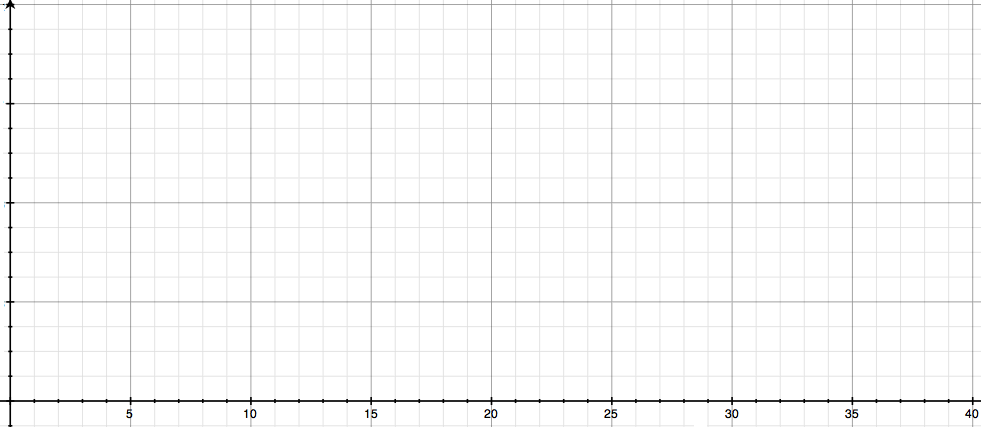
\includegraphics[width=12cm, height=6cm]{Tolerance_crystals_axis2.png}
    \end{problem}
    
    %%Part2d
    \begin{problem}{\textbf{\#2d:}}
    \textbf{Your answer to this question should be typed or written in a separate document and labeled as Problem 2d.}
    
    \textbf{Label} interval of temperature ($T$-interval) that can be tolerated for proper crystal growth. Your label should be placed on the $T$-axis and should be titled ``$T$-Interval''
    
	\textbf{Label} the $w$-interval you found in part (b) for input power that corresponds to the given $T$-interval. Your label should be placed on the $w$-axis and should be titled ``$w$-Interval''
    \end{problem}
    
    %%Part 2e
    \begin{problem}{\textbf{\#2e:}}
    \textbf{Your answer to this question should be typed or written in a separate document and labeled as Problem 2e.}
    After more experiments, it is determined that the temperature must actually be kept closer to 200 °C than $\pm 1^\circ$C for proper crystal growth.  Can we repeat the process in \#2b to find an acceptable power interval even if the temperature must be kept arbitrarily close to $200^\circ$C?  Explain why or why not by referencing the graph you produced in \#2c and \#2d.
    \end{problem}
    
\end{problem}

%%PROBLEM 3%%
\begin{problem}{\textbf{\#3:}}
\textbf{Your answer to this question should be typed or written in a separate document and labeled as Problem 3. You can add to the document containing your answers from problems 1 and 2.}

For problems 1 and 2 you had to find an interval of input values that would satisfy an arbitrarily small interval of output values (if the word ‘‘arbitrary’’ is throwing you off, chat with your instructor). Can this be done for any function? If yes, explain why. If not, provide a graph or function of a counter example and explain why it is a counter example. \\ A counterexample is an example of a function for which the ``if'' part of the statement is true, but the ``then'' part is false. A counterexample in this instance is a function AND an interval of output values for which you cannot find a corresponding interval of input values, as you have been able to in \#1 and \#2..
\end{problem}

Note: For the following problems, you may find it helpful to look at a graph of the functions.

%%PROBLEM 4 - cos (pi/x)%%
\begin{problem}{\textbf{\#4: }}{\textbf{\textit{An Investigation with tables. Be careful; tables can be misleading! }}}
Use $\displaystyle f(x)=\cos\left(\frac{\pi}{x}\right)$ to fill in the following three tables.
Use the Desmos calculator widget below to compute your answers. Report any non-terminating values to 8 decimal places.

\[
\graph[panel]{cos(\frac{\pi}{0.1})}
\]

\begin{tabular}{|c|c|}

\hline
		$x$ & $\cos\left(\frac{\pi}{x}\right)$\\
		
        $0.1$ & $\answer{1}$\\
		
		$0.01$ & $\answer{1}$\\
		
		$0.001$ & $\answer{1}$\\
		
		$0.0001$ & $\answer{1}$\\
		
		$0.00001$ & $\answer{1}$ \\
		
		$0.000001$ & $\answer{1}$ \\

		
\end{tabular}

\bigskip
\bigskip

\begin{tabular}{|c|c|}

\hline
		$x$ & $\cos\left(\frac{\pi}{x}\right)$\\
		
        $0.15$ & $\answer{-0.5}$\\
		
		$0.015$ & $\answer{-0.5}$\\
		
		$0.0015$ & $\answer{-0.5}$\\
		
		$0.00015$ & $\answer{-0.5}$\\
		
		$0.000015$ & $\answer{-0.5}$ \\
		
		$0.0000015$ & $\answer{-0.5}$ \\

		
\end{tabular}

\bigskip
\bigskip

\begin{tabular}{|c|c|}

\hline
		$x$ & $\cos\left(\frac{\pi}{x}\right)$\\
		
        $-0.2$ & $\answer{-1}$\\
		
		$-0.03$ & $\answer{-0.5}$\\
		
		$-0.004$ & $\answer{1}$\\
		
		$-0.0005$ & $\answer{1}$\\
		
		$-0.00006$ & $\answer{-0.5}$ \\
		
		$-0.000007$ & $\answer[tolerance=0.0000001]{-0.9009688673}$ \\

		
\end{tabular}



    %%Part 4a
  %  \begin{problem}{\textbf{\#4a}}
  %  From the above results, what do you conclude about $\displaystyle\lim_{x\rightarrow 0}\cos\left(\frac{\pi}{x}\right)$? Explain in terms of what it means for a function to have a limit (or not to have a limit) how the values in the tables support your conclusion.
   % \end{problem}
    
\end{problem}


%%PROBLEM 5 - sin(1/x)%%
\begin{problem}{\textbf{\#5:}}
Use $\displaystyle f(x)=\sin\left(\frac{1}{x}\right)$ to answer the following.
Let's make a table of values. Use the Desmos calculator widget below to compute your answers to \textbf{\underline{8 decimal places}}.

\[
\graph[panel]{sin(1/-1)}
\]

%%Part 5a
\begin{problem}{\textbf{\#5a:}}

\begin{tabular}{|c|c|}

\hline
		$x$ & $f(x)$\\
		
        $-0.1$ & $\answer[tolerance=0.000000001]{0.54402111}$\\
		
		$-0.01$ & $\answer[tolerance=0.000000001]{0.50636564}$\\
		
		$-0.001$ & $\answer[tolerance=0.000000001]{-0.82687954}$\\
		
		$-1\times10^{-4}$ & $\answer[tolerance=0.000000001]{0.30561439}$\\
		
		$-1\times10^{-5}$ & $\answer[tolerance=0.000000001]{-0.03574880}$ \\
		
		$-1\times10^{-6}$ & $\answer[tolerance=0.000000001]{0.34999350}$ \\
		
		$-1\times10^{-7}$ & $\answer[tolerance=0.000000001]{-0.42054779}$ \\
		
		$-1\times10^{-8}$ & $\answer[tolerance=0.000000001]{-0.93163903}$ \\
		
        $0$ & \wordChoice{\choice{0}\choice{infinity}\choice[correct]{undefined}}\\
        
		$2\times10^{-8}$ & $\answer[tolerance=0.000000001]{0.82564674}$ \\
		
		$2\times10^{-7}$ & $\answer[tolerance=0.000000001]{-0.97654247}$ \\
		
		$2\times10^{-6}$ & $\answer[tolerance=0.000000001]{0.17783120}$ \\
		
		$2\times10^{-5}$ & $\answer[tolerance=0.000000001]{-0.99984019}$ \\
		
		$2\times10^{-4}$ & $\answer[tolerance=0.000000001]{-0.98796644}$ \\
		
		$0.002$ & $\answer[tolerance=0.000000001]{-0.46777181}$ \\
		
		$0.02$ & $\answer[tolerance=0.000000001]{-0.26237485}$ \\
		
		$0.2$ & $\answer[tolerance=0.000000001]{-0.95892427}$ \\
		
\end{tabular}
\end{problem}



%%Part 5b
\begin{problem}{\textbf{\#5b:}}

Plot the graph of $f(x)=\sin\left(\frac{1}{x}\right)$ on the $x$-window $[-0.5,0.5]$. You can use the Desmos widget to generate graphs. 

\textbf{Provide a detailed print-out of the graph and attach it to the questions you have written in a separate document. Label the graph as 4c.}

\begin{hint}
Click on the wrench icon in the Desmos widget to adjust the values on the axes.
\end{hint}


\end{problem}

%%Part 5c
\begin{problem}{\textbf{\#5c:}}

Plot the graph of $f(x)=\sin\left(\frac{1}{x}\right)$ on the $x$-window $[-0.1,0.1]$. You can use the Desmos widget to generate graphs. 

\textbf{Provide a detailed print-out of the graph and attach it to the questions you have written in a separate document. Label the graph as 4d.}

\end{problem}

\[
\graph[panel]{}
\]

\end{problem}

%%DISCUSSION BEHAVIOR%%

\underline{\hspace{5in}}

An example of talking about ``\textbf{\underline{behavior}}'':

\[
\graph[panel]{1-x^2}
\]

Look at the graph of $f(x)=1-x^2$ in the desmos window. 

When discussing the \underline{\textbf{behavior}} of $f(x)=1-x^2$, we say that as $x$ tends toward 0 from either side, the function values increase from more negative values to 1.

\underline{\hspace{5in}}

%%PROBLEM 6
\begin{problem}{\textbf{\#6:}}
Based on your work in problems 4 and 5 and the behavior of the functions, what can you conclude about the behavior of $\sin\left(\frac{1}{x}\right)$ and $\cos\left(\frac{\pi}{x}\right)$ as $x$ approaches 0?

Your explanation should be 1-3 sentences. Be sure to reference the data tables and/or graphs to support your explanation.

\end{problem}





























\end{document}

